\section{Introduction}

% \textcolor{red}{Start from applications, rather than from high-productivity hardware design. Just one sentence should be enough.}
Deep neural networks (DNNs) have gained major interest in recent years in application domains ranging from computer vision, to machine translation, to robotic manipulation.
However, running modern, accurate DNNs with high performance and low energy consumption is often challenging without dedicated accelerators which are difficult and expensive to design.
The demand for cheaper, high-productivity hardware design has motivated a number
of research efforts to develop highly-parameterized and modular hardware
generators for DNN
accelerators and other hardware building blocks~\cite{moreau2018, venkatesan2019magnet,polysa,zhang2018,automated-systolic-cnn-fpgas,deepburning,hybrid-dnn}.
While the hardware generator efforts make it easier to instantiate a DNN accelerator,
they primarily focus on the design of the accelerator component itself, rather than taking into consideration the system-level parameters that determine the overall SoC and the full software stack.
Some industry perspectives have advocated for a more
holistic exploration of DNN accelerator development and deployment~\cite{datacenter-facebook,edge-facebook,ai-tax-hpca}.
However, existing DNN generators have little support for a full-stack programming interface which provides both high and low-level control of the accelerator, and little support for full SoC integration, making it challenging to evaluate system-level implications. 

In this work, we present Gemmini, an open-source, full-stack DNN accelerator
generator for DNN workloads, enabling end-to-end, full-stack implementation and evaluation
of custom hardware accelerator systems for rapidly evolving DNN workloads.
Gemmini's hardware template and parameterization allows users to tune the
hardware design options across a broad spectrum spanning performance, efficiency,
and extensibility.
Unlike existing DNN accelerator generators that focus on standalone accelerators, Gemmini also provides a complete solution spanning both the hardware and software stack, and a complete SoC integration that is compatible with the RISC-V ecosystem.
In addition, Gemmini implements a multi-level software stack with an easy-to-use programming interface to support different programming requirements, as well as tight integration with Linux-capable SoCs which enable the execution of any arbitrary software.

% Gemmini implements a simple programming interface which lends itself to
% customization and easy modification, as well as tight integration with
% Linux-capable SoCs, which enable the execution of any arbitrary software.
% In addition, Gemmini provides a multi-level software stack with an easy-to-use programming interface to support different programming requirements.
%enabling direct execution of DNN models from a high-level description in the ONNX
%format, an open exchange format built to represent DNN models across different frameworks~\cite{onnx}.

%==============Table 1===============================
\begin{table*}[t]
% \begin{tabularx}{\linewidth}{ l | >{\centering}p{3cm} | cccccccc }
\begin{tabularx}{\linewidth}{ c | >{\centering}p{2.5cm} | cccccccc }
\toprule
% \cmidrule(l){2-9}
& Property
% & \makecell{NVDLA\\\cite{nvdla}}
& NVDLA%\cite{nvdla}
& VTA%\cite{moreau2018}
& PolySA%\cite{polysa}
& DNNBuilder%\cite{zhang2018}
& MAGNet%\cite{venkatesan2019magnet}
& DNNWeaver%\cite{dnnweaver}
& MAERI%\cite{maeri-asplos2018}
& Gemmini \\
\midrule
\multirow{4}{*}{\makecell{Hardware\\Architecture\\Template}} & Datatypes & Int/Float & Int & Int & Int  & Int & Int & Int & Int/Float \\
& Dataflows & \xmark & \xmark & \cmark & \cmark & \cmark & \cmark & \cmark & \cmark \\ 
& \makecell{Spatial Array} & vector & vector & systolic & systolic & vector & vector & vector & vector/systolic \\
& Direct Convolution & \cmark & \xmark & \xmark & \cmark &  \cmark & \cmark & \cmark & \cmark \\
\hline
\multirow{2}{*}{\makecell{Programming\\Support}} & Software Ecosystem & Compiler & TVM &  SDAccel & Caffe & C & Caffe & Custom & ONNX/C \\ 
& Virtual Memory & \xmark & \xmark & \xmark & \xmark & \xmark & \xmark & \xmark & \cmark \\
\hline
\multirow{2}{*}{\makecell{System\\Support}} & \makecell{Full SoC} & \xmark & \xmark & \xmark & \xmark & \xmark & \xmark & \xmark & \cmark \\
& \makecell{OS Support} & \cmark & \cmark & \xmark & \xmark & \xmark & \xmark & \xmark & \cmark \\ 

\bottomrule
\end{tabularx}
\caption{Comparison of DNN accelerator generators.}
\label{tab:generator-comparison}
\vspace{-0.2in}
\end{table*}


%==============End of Table 1===============================

Gemmini-generated accelerators have been successfully fabricated in both TSMC
$16nm$ FinFET and Intel $22nm$ FinFET Low Power (22FFL) process technologies, demonstrating that they can be physically realized.
In addition, our evaluation shows that Gemmini-generated accelerators deliver comparable
performance to a state-of-the-art, commercial DNN
accelerator~\cite{nvdla-hotchips} with a similar set of hardware configurations and achieve up to 2,670x speedup with respect to a baseline CPU.
%Our case studies demonstrate how 
Gemmini's fully-integrated, full-stack flow enables users to co-design the accelerator, application, and system all at once, opening up new research opportunities for future DL SoC integration. Specifically, in our Gemmini-enabled case studies, we demonstrate how designers can use Gemmini to optimize virtual address translation mechanisms for DNN accelerator workloads, and to partition memory resources in a way that balances the different compute requirements of different layer types within a DNN.

% Our case studies further show the benefits of Gemmini's fully-integrated, full-stack flow and the importance of system-level considerations in accelerator design, such as the provisioning of memory resources in an SoC, or the design of a virtual memory translation scheme to alleviate programmer burden while preserving high memory bandwidth.

In brief, this work makes the following contributions:

\begin{enumerate}
\item We build Gemmini, an open-source, full-stack DNN accelerator design
infrastructure to enable systematic evaluation of deep-learning architectures.
Specifically, Gemmini provides a flexible hardware template, a multi-layered
software stack, and an integrated SoC environment (Section~\ref{sec:generator}).

\item We perform rigorous evaluation of Gemmini-generated accelerators using FPGA-based performance measurement and commercial ASIC synthesis flows for performance and efficiency analysis. Our evaluation demonstrates that Gemmini-generated accelerators deliver comparable performance compared to state-of-the-art, commercial DNN accelerators (Section~\ref{sec:evaluation}). %\textcolor{red}{(Did we really compare efficiency, or just performance?)}

\item We demonstrate that the Gemmini infrastructure enables system-accelerator co-design of SoCs running DNN workloads, including the design of efficient virtual-address translation schemes for DNN accelerators and the provisioning of memory resources in a shared cache hierarchy (Section~\ref{sec:casestudies}).
\end{enumerate}

\begin{figure}[t]
    \centering
    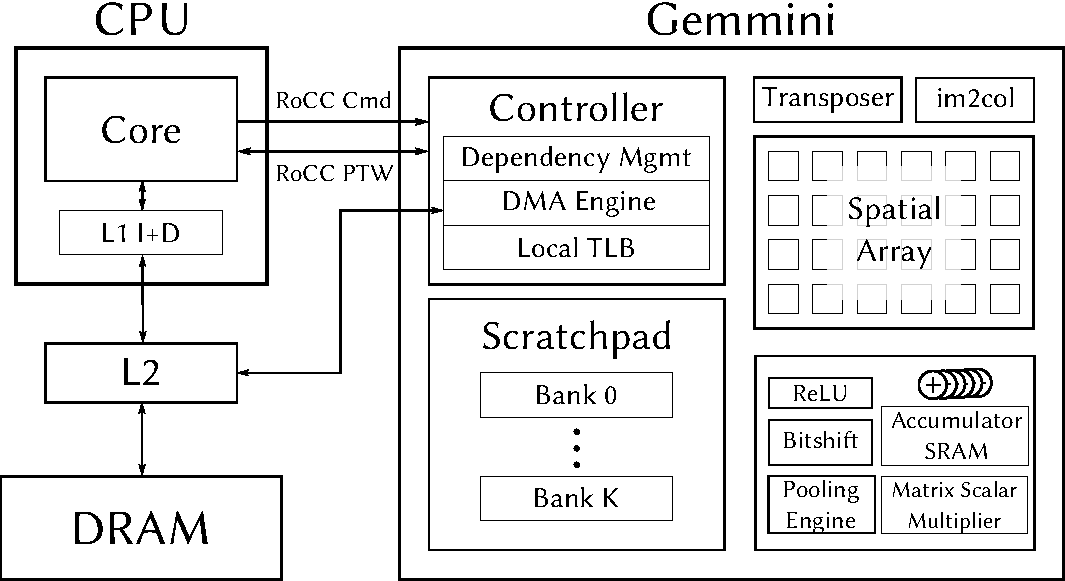
\includegraphics[width=0.9\linewidth]{fig/systolic_arch_system.pdf}
    \caption{Gemmini hardware architectural template overview.}
    \vspace{-0.3cm}
    \label{fig:arch-template}
    \vspace{-0.1in}
\end{figure}

%========OLD TEXT BELOW================

%\textcolor{red}{Introduce Gemmini here. Explain how it addresses the limitations earlier. In one concluding sentence, describe our performance/power.} Gemmini provides a push button flow from ONNYX representations to ready to tape-out design with all the necessary software and hardware libraries. It provides flexibility in the generated hardware and in the programming model allowing users to easily modify the underlying hardware configurations, add more hardware units and extend the ISA with new instructions. Gemmini also provides system level integration, and achieves comparable results to the industry standard NVDLA systolic array accelerator~\cite{}.

% Chipyard~\cite{chipyard} is a framework for designing and evaluating full-system hardware. It includes in-order, out-of-order RISC-V, and vector processors, and an accelerator for SHA3 hash function. In this work we extend the Chipyard framework with Gemmini: a systolic array generator.  A large portion of DNN accelerators produced by major vendors such as Google~\cite{tpu}, Samsung~\cite{samsung} and Tesla~\cite{bannon2019accelerated} have used systolic array architectures for matrix multiplication and convolution operations.

% Gemmini plugs-in within the tile interface of the Rocket Chip SoC generator ecosystem and the Chipyard integrated SoC research and development framework. As such, it integrates with a broad set of open-source heterogeneous SoC components and devices, including UARTs, GPIOs, JTAGs, shared-cache memory systems, and various accelerators. These components include the open-source SiFive inclusive L2 cache, the Hwacha vector accelerator [13], and BOOM.

%\textcolor{red}{Move this table and description of it to the Background section.} Figure~\ref{} shows the advantages of Gemmini as compared to NVDLA and VTA~\cite{} and where it is positioned in terms of flexibility, system level integration and performance.

% Gemmini is gaining widespread adoption in research labs. More than 30 students, both graduate and undergraduate, including ones with very little hardware experience, were able to take advantage of this in Berkeley's Hardware For Machine Learning class~\cite{} and design new features. In \cite{PekingTVM} Gemmini was integrated with TVM~\cite{TVM} allowing for automatic code generation and autotuning.

%\textcolor{red}{Describe case studies here, with one sentence each.} We perform three case studies on Gemmini and explore its flexibility, system-level integration, and performance (in terms of execution time, and energy consumption).
% Our evaluation includes booting Linux on Gemmini, running real cycle-accurate simulations on AWS FPGA instances using Firesim~\cite{karandikar2018firesim}, exploring multiple hardware configurations, programming models, and host co-processors and experimenting with a wide range of DNNs. 
%Finally, we fabricated two test systems-on-chip Gemmini designs in TSMC 16nm and Intel 22FFL process technologies.
%Our main contributions are:

% (programming model fine grained and coarse grained instructons and hardware), system level integration, comparable NVDLA + plot

% We have the whole package:
%     * push button flow from high level software to ready to tapeout flow.
%     * Software compilation
%     * Real system integration from
%     * FPGA-accelerated simulation to get cycle-accurate performance
%     * Physical design

%Hardware acceleration requires specialized hardware. The non-recurring
%engineering (NRE) costs of specialized hardware limit it's adoption to a small
%number of high-value applications. 
%%\textcolor{red}{Change this paragraph instead to focus on WHY we need generators.} With the demise of Dennard's scaling and the end of Moore's law, hardware customization became the go-to approach for handling the exacerbating compute demand. \textcolor{red}{Transition missing here, e.g. hardware customization is extremely difficult.} 
%Hardware generators~\cite{bora_generators, bora_generators2} are an attractive approach to lower the NRE costs of custom hardware. Rather than designing instances from scratch for each new application, designing highly-parameterized and modular instance generators which capture the main computational properties and control flow of hardware instances, but allow them to be tailored and customized to specific application use-cases. \textcolor{red}{(This previous sentence is too long. The discussion is also too general, so we should tie it closer to DNNs. Make a case for DNN generators in particular, rather than just generators.)}
%DNN accelerators are a prime use-case for hardware generators.
%Although DNN computational kernels may stay the same across workloads, characteristics such as layer dimensions or model size impact how workloads are optimally scheduled and mapped to any particular hardware accelerator, lending themselves to further accelerator customization. 
%By tailoring the parameters of a hardware generator to a target applications based on pre-silicon application-specific design-space-exploration, designer can extract maximal efficiency from an accelerator integrated with an application, while minimizing NRE costs for that particular application. 

%This paper describes the architecture and features of the Gemmini generator
%hardware and software tools together with a performance evaluation.
